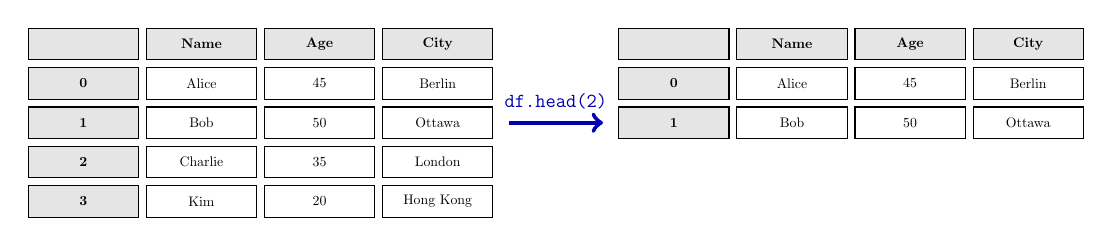
\begin{tikzpicture}[scale=0.5, transform shape,
    cell/.style={
        draw,
        minimum width=2.8cm,
        minimum height=0.8cm,
        align=center
    },
    header/.style={
        cell,
        fill=gray!20,
        font=\bfseries
    }
]

%%%%%%%%%%%%%%%%%%%%%%%%
% DataFrame original
%%%%%%%%%%%%%%%%%%%%%%%%

% --- Headers ---
\node[header] (h0) at (0,0) {};
\node[header] (h1) at (3,0) {Name};
\node[header] (h2) at (6,0) {Age};
\node[header] (h3) at (9,0) {City};

% --- Row 0 ---
\node[header] at (0,-1) {0};
\node[cell] at (3,-1) {Alice};
\node[cell] at (6,-1) {45};
\node[cell] at (9,-1) {Berlin};

% --- Row 1 ---
\node[header] at (0,-2) {1};
\node[cell] at (3,-2) {Bob};
\node[cell] at (6,-2) {50};
\node[cell] at (9,-2) {Ottawa};

% --- Row 2 ---
\node[header] at (0,-3) {2};
\node[cell] at (3,-3) {Charlie};
\node[cell] at (6,-3) {35};
\node[cell] at (9,-3) {London};

% --- Row 3 ---
\node[header] at (0,-4) {3};
\node[cell] at (3,-4) {Kim};
\node[cell] at (6,-4) {20};
\node[cell] at (9,-4) {Hong Kong};

%%%%%%%%%%%%%%%%%%%%%%%%
% Flecha df.head(2)
%%%%%%%%%%%%%%%%%%%%%%%%

\draw[->, ultra thick, blue!70!black]
    (10.8,-2)
    to[out=0,in=180]
    node[midway, above=6pt, font=\ttfamily\Large, text=blue!70!black]
    {df.head(2)}
    (13.2,-2);

%%%%%%%%%%%%%%%%%%%%%%%%
% Resultado df.head(2)
%%%%%%%%%%%%%%%%%%%%%%%%

% --- Headers ---
\node[header] at (15,0) {};
\node[header] at (18,0) {Name};
\node[header] at (21,0) {Age};
\node[header] at (24,0) {City};

% --- Row 0 ---
\node[header] at (15,-1) {0};
\node[cell] at (18,-1) {Alice};
\node[cell] at (21,-1) {45};
\node[cell] at (24,-1) {Berlin};

% --- Row 1 ---
\node[header] at (15,-2) {1};
\node[cell] at (18,-2) {Bob};
\node[cell] at (21,-2) {50};
\node[cell] at (24,-2) {Ottawa};

\end{tikzpicture}
